\documentclass[11pt]{article}
\usepackage[utf8]{inputenc}
\usepackage{fullpage,amsmath,amsthm,enumerate}
\usepackage[citecolor=blue,linkcolor=blue,colorlinks=true]{hyperref}
\usepackage{tikz}
\usepackage{graphicx}
\usepackage{xcolor}  % To color a text in 
\usepackage{multicol} % For multiple columns
\usepackage{caption}
\usepackage{subcaption}
\counterwithin{table}{subsection}
\counterwithin{figure}{subsection}

% Theorems
\newtheorem{theorem}{Theorem}
\newtheorem{lemma}{Lemma}

% Commands
\newcommand{\calF}{$\mathcal{F}$}
\newcommand{\set}[1]{\{ #1 \}}
\newcommand{\zon}{$\{0,1\}^n$}
\newcommand{\zo}{$\{0,1\}$}

\title{Classification Task\\
Report}
\author{Reetwik Das}

\begin{document}
\maketitle
\newpage
\tableofcontents
\listoftables
\listoffigures

\newpage 

\section{Dataset 1a}
\subsection{K-nearest neighbours classifier}
Hyperparameters $K = \{1,7,15\}$
\begin{table}[h!]
\label{tab:tab1.1.1}
\begin{center}
\begin{tabular}{|l|c|c|c|}
\hline
\textbf{K } & \textbf{Training Dataset} & \textbf{Validation Dataset} &\textbf{Test Dataset}\\
\hline
$1$ & 100 & 100 & 100\\
\hline
$7$ & 100 & 100 & 100\\
\hline
$15$ & 100 & 100 & 100\\
\hline
\end{tabular}
\caption{Classification accuracy of KNN classifier on Dataset 1a}
\end{center}
\end{table}

As we can see from the table above the model with the best performance on the test data is with  K=1 with an accuracy of 100\% (same accuracy with least computation cost).
\begin{figure}[h]
\centering
	\begin{subfigure}[b]{0.45\textwidth}
	\centering
	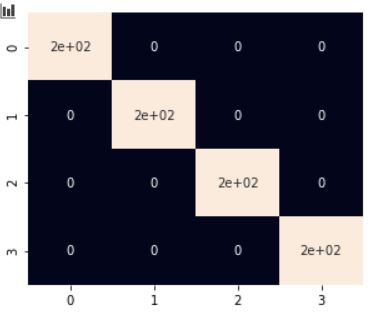
\includegraphics[scale=0.6]{dataset1a_knn_hm_train.jpg}
	\caption{for Training data}
	\label{fig:fig2.2.3.1}
	\end{subfigure}
	\hfill
	\begin{subfigure}[b]{0.45\textwidth}
	\centering
	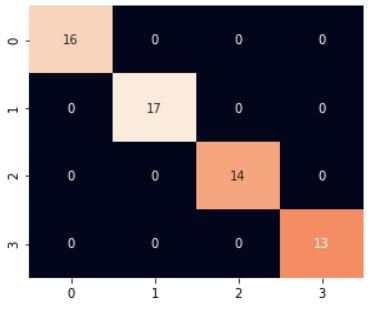
\includegraphics[scale=0.6]{dataset1a_knn_hm_test.jpg}
	\caption{for Test data}
	\label{fig:fig2.2.3.2}
	\end{subfigure}
\caption{Confusion matrix for datatset 1a using KNN classifier,  $K=1$}
\label{fig:fig1.2.1}
\end{figure}

\begin{figure}[h]
\centering
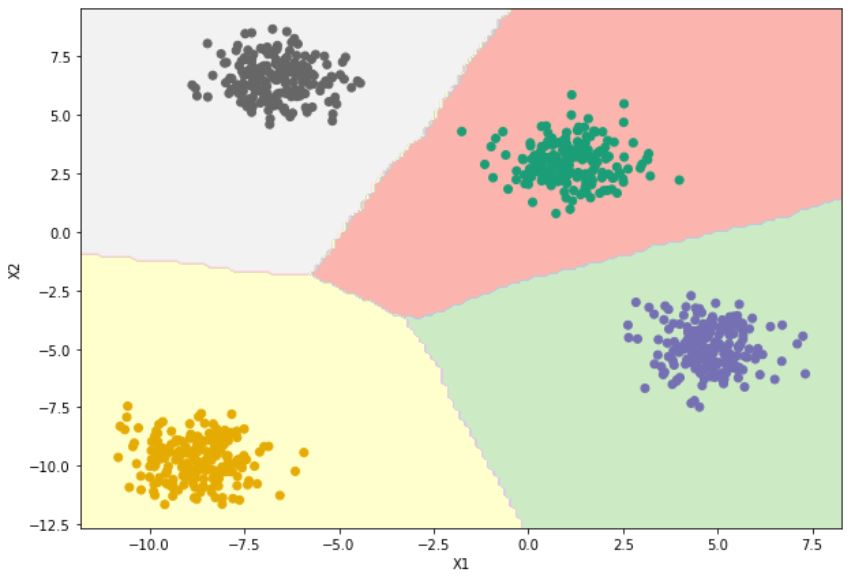
\includegraphics[scale=0.4]{dataset1a_knn.jpg}	
\caption{Decision region plots superposed with training examples for datatset 1a using KNN classifier, $K=1$}
\label{fig:fig1.1.1}
\end{figure}

\newpage
\subsection{Naive bayes Classifier, covariance matrix for all the classes is $\sigma^2I$}

\begin{table}[h!]
\label{tab:tab1.1.1}
\begin{center}
\begin{tabular}{|c|c|c|}
\hline
\textbf{Training Dataset} & \textbf{Validation Dataset} &\textbf{Test Dataset}\\
\hline
100 & 100 & 100\\
\hline
\end{tabular}
\caption{Classification accuracy of Naive bayes classifier on Dataset 1a, the covariance matrices are same and $=\sigma^2I$}
\end{center}
\end{table}

\begin{figure}[h]
\centering
	\begin{subfigure}[b]{0.45\textwidth}
	\centering
	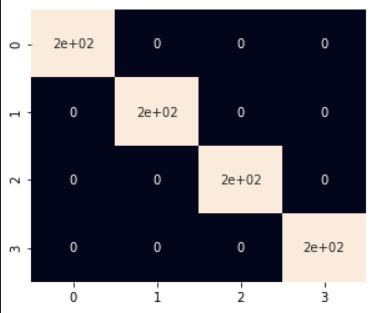
\includegraphics[scale=0.6]{dataset1a_nb_sigmaI_hm_train.jpg}
	\caption{for Training data}
	\label{fig:fig2.2.3.1}
	\end{subfigure}
	\hfill
	\begin{subfigure}[b]{0.45\textwidth}
	\centering
	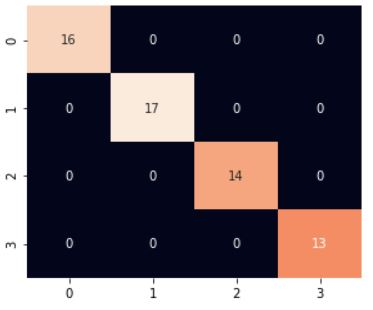
\includegraphics[scale=0.6]{dataset1a_nb_sigmaI_hm_test.jpg}
	\caption{for Test data}
	\label{fig:fig2.2.3.2}
	\end{subfigure}
\caption{Confusion matrix for datatset 1a using Naive bayes classifier, the covariance matrices are same and $= \sigma^2 I$}
\label{fig:fig1.2.1}
\end{figure}

\begin{figure}[h]
\centering
	\begin{subfigure}[b]{0.45\textwidth}
	\centering
	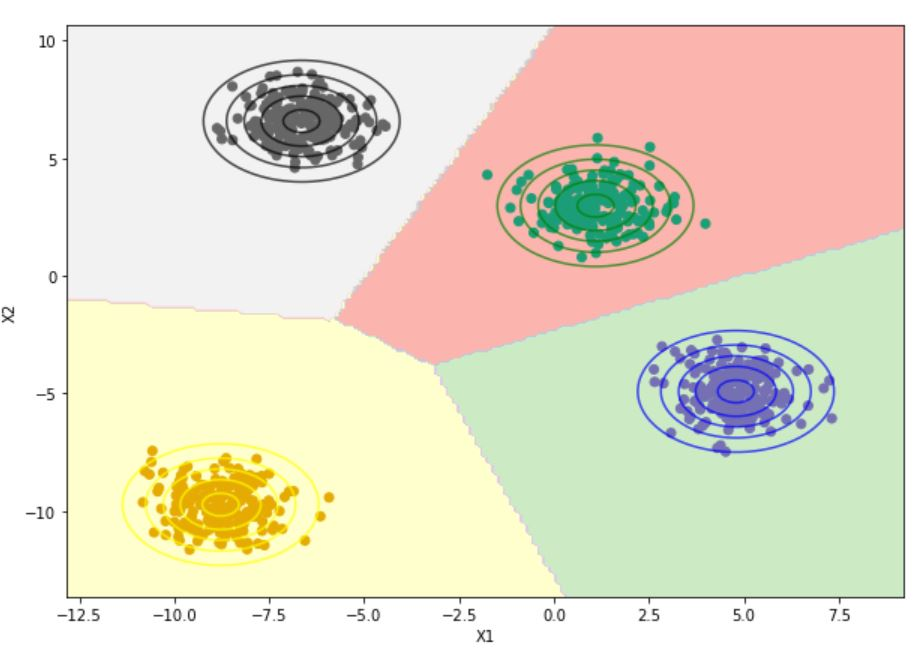
\includegraphics[scale=0.3]{dataset1a_sigmaI_nb_2D.jpg}
	\caption{Decision region plots superposed with training examples}
	\label{fig:fig2.2.3.1}
	\end{subfigure}
	\hfill
	\begin{subfigure}[b]{0.45\textwidth}
	\centering
	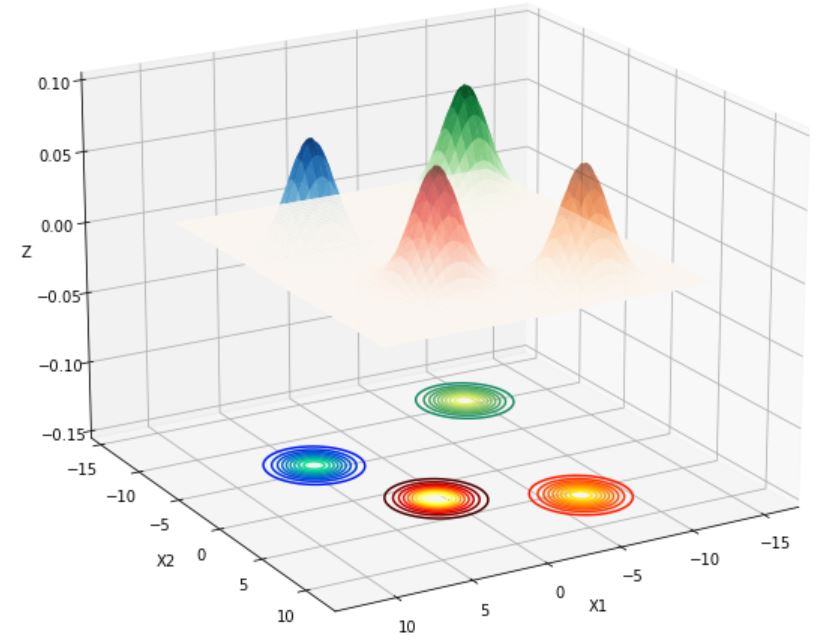
\includegraphics[scale=0.3]{dataset1a_sigmaI_nb_3D.jpg}
	\caption{Plots of the level curves}
	\label{fig:fig2.2.3.2}
	\end{subfigure}
\caption{Plots for datatset 1a using Naive bayes classifier, the covariance matrices are same and $= \sigma^2 I$}
\label{fig:fig1.2.1}
\end{figure}

\newpage
\subsection{Naive bayes Classifier, covariance matrix for all the classes is $C$}

\begin{table}[h!]
\label{tab:tab1.1.1}
\begin{center}
\begin{tabular}{|c|c|c|}
\hline
\textbf{Training Dataset} & \textbf{Validation Dataset} &\textbf{Test Dataset}\\
\hline
100 & 100 & 100\\
\hline
\end{tabular}
\caption{Classification accuracy of Naive bayes classifier on Dataset 1a, the covariance matrices are same $= C$}
\end{center}
\end{table}

\begin{figure}[h]
\centering
	\begin{subfigure}[b]{0.45\textwidth}
	\centering
	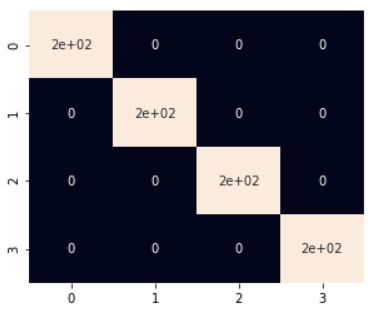
\includegraphics[scale=0.6]{dataset1a_nb_sameC_hm_train.jpg}
	\caption{for Training data}
	\label{fig:fig2.2.3.1}
	\end{subfigure}
	\hfill
	\begin{subfigure}[b]{0.45\textwidth}
	\centering
	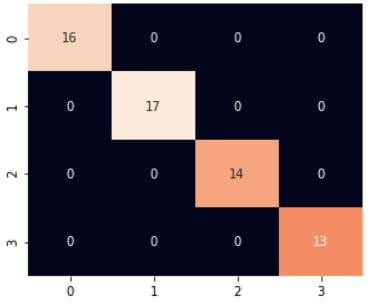
\includegraphics[scale=0.6]{dataset1a_nb_sameC_hm_test.jpg}
	\caption{for Test data}
	\label{fig:fig2.2.3.2}
	\end{subfigure}
\caption{Confusion matrix for datatset 1a using Naive bayes classifier, the covariance matrices are same $= C$}
\label{fig:fig1.2.1}
\end{figure}

\begin{figure}[h]
\centering
	\begin{subfigure}[b]{0.45\textwidth}
	\centering
	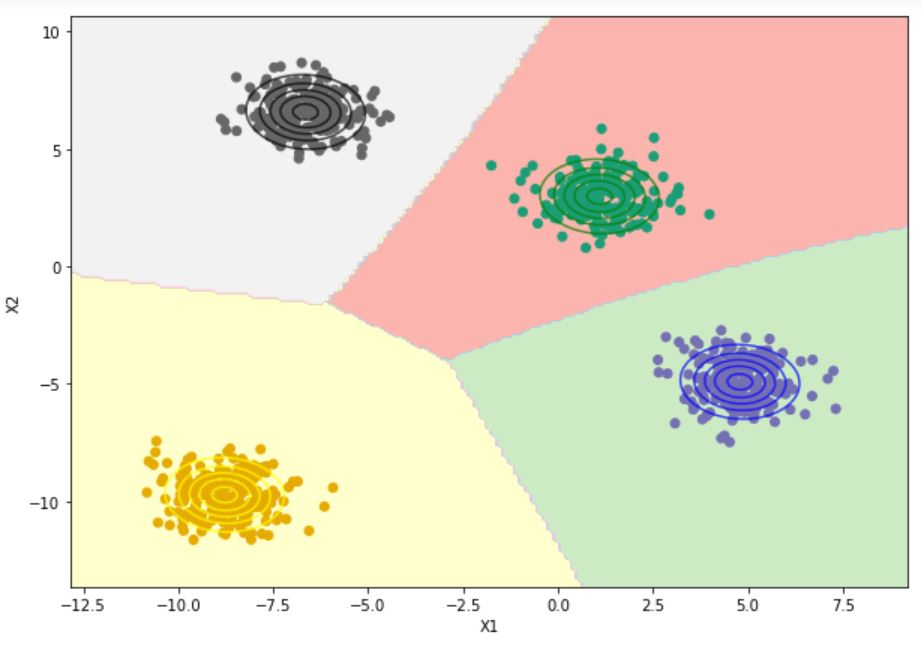
\includegraphics[scale=0.3]{dataset1a_sameC_nb_2D.jpg}
	\caption{Decision region plots superposed with training examples}
	\label{fig:fig2.2.3.1}
	\end{subfigure}
	\hfill
	\begin{subfigure}[b]{0.45\textwidth}
	\centering
	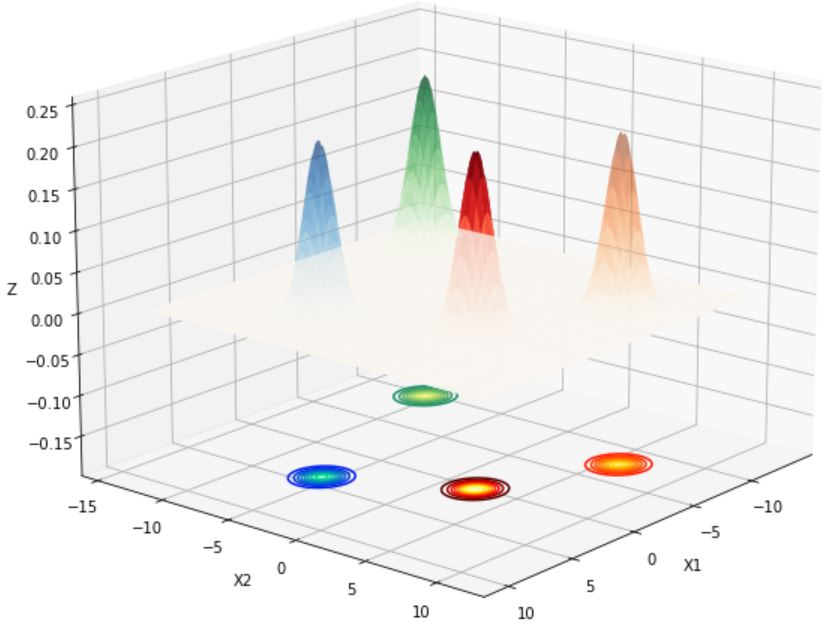
\includegraphics[scale=0.3]{dataset1a_sameC_nb_3D.jpg}
	\caption{Plots of the level curves}
	\label{fig:fig2.2.3.2}
	\end{subfigure}
\caption{Plots for datatset 1a using Naive bayes classifier, the covariance matrices are same $= C$ }
\label{fig:fig1.2.1}
\end{figure}

\newpage
\subsection{Naive bayes Classifier, covariance matrix for all the classes is different}

\begin{table}[h!]
\label{tab:tab1.1.1}
\begin{center}
\begin{tabular}{|c|c|c|}
\hline
\textbf{Training Dataset} & \textbf{Validation Dataset} &\textbf{Test Dataset}\\
\hline
100 & 100 & 100\\
\hline
\end{tabular}
\caption{Classification accuracy of Naive bayes classifier on Dataset 1a,  the covariance matrices are different}
\end{center}
\end{table}

\begin{figure}[h]
\centering
	\begin{subfigure}[b]{0.45\textwidth}
	\centering
	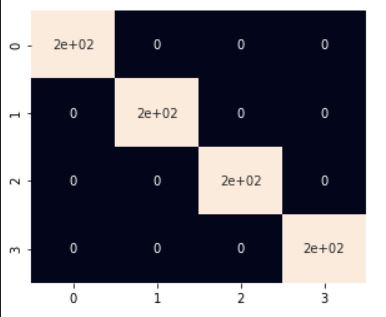
\includegraphics[scale=0.6]{dataset1a_nb_differentC_hm_train.jpg}
	\caption{for Training data}
	\label{fig:fig2.2.3.1}
	\end{subfigure}
	\hfill
	\begin{subfigure}[b]{0.45\textwidth}
	\centering
	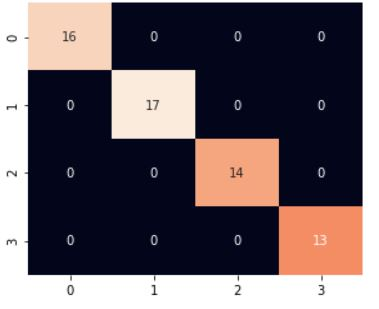
\includegraphics[scale=0.6]{dataset1a_nb_differentC_hm_test.jpg}
	\caption{for Test data}
	\label{fig:fig2.2.3.2}
	\end{subfigure}
\caption{Confusion matrix for datatset 1a using Naive bayes classifier,  the covariance matrices are different}
\label{fig:fig1.2.1}
\end{figure}

\begin{figure}[h]
\centering
	\begin{subfigure}[b]{0.45\textwidth}
	\centering
	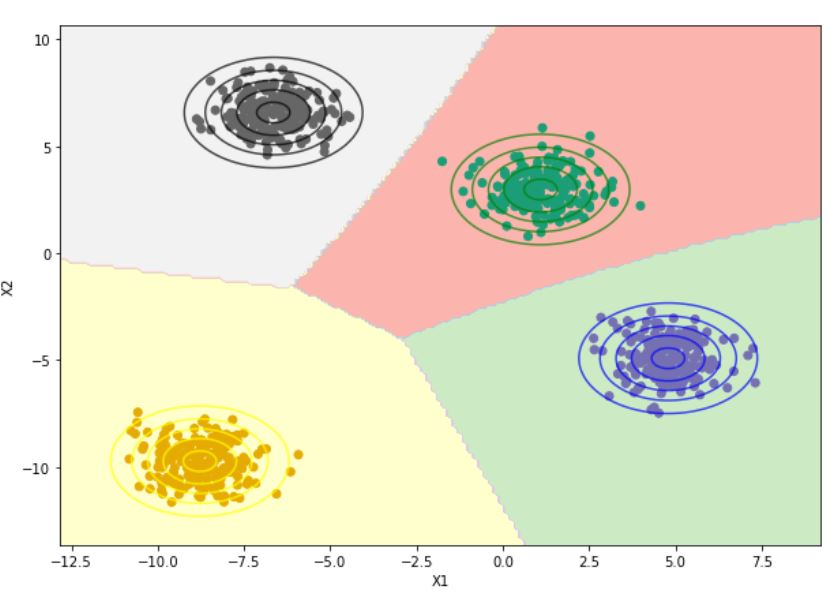
\includegraphics[scale=0.3]{dataset1a_differentC_nb_2D.jpg}
	\caption{Decision region plots superposed with training examples}
	\label{fig:fig2.2.3.1}
	\end{subfigure}
	\hfill
	\begin{subfigure}[b]{0.45\textwidth}
	\centering
	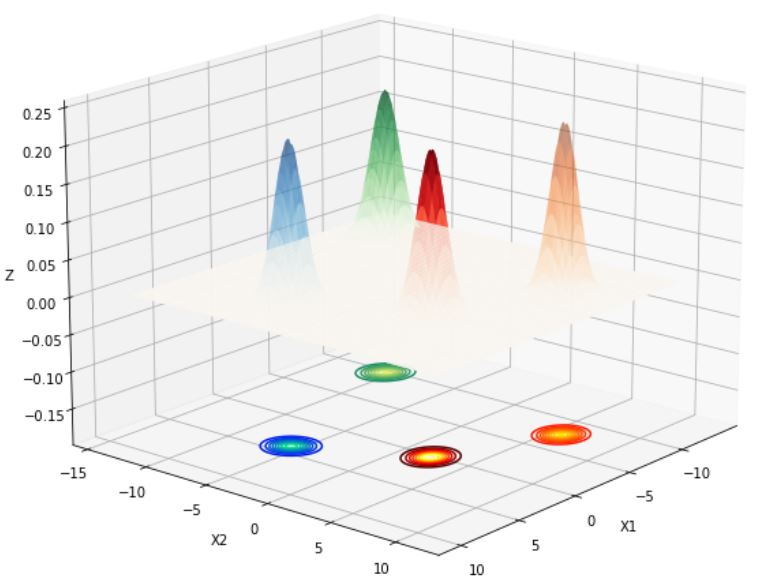
\includegraphics[scale=0.3]{dataset1a_differentC_nb_3D.jpg}
	\caption{Plot of level curves}
	\label{fig:fig2.2.3.2}
	\end{subfigure}
\caption{Plots for datatset 1a using Naive bayes classifier, the covariance matrices are different }
\label{fig:fig1.2.1}
\end{figure}

We observed that since all the classes are well separated all the classification approaches gave us very good results.
\newpage

\section{Dataset 1b}
\subsection{K-nearest neighbours classifier}
Hyperparameters $K = \{1,7,15\}$
\begin{table}[h!]
\label{tab:tab1.1.1}
\begin{center}
\begin{tabular}{|l|c|c|c|}
\hline
\textbf{K } & \textbf{Training Dataset} & \textbf{Validation Dataset} &\textbf{Test Dataset}\\
\hline
$1$ & 100 & 100 & 100\\
\hline
$7$ & 100 & 100 & 100\\
\hline
$15$ & 99.67 & 100 & 100\\
\hline
\end{tabular}
\caption{Classification accuracy of KNN classifier on Dataset 1b}
\end{center}
\end{table}

As we can see from the table above the model with the best performance on the test data is with  K=1 with an accuracy of 100\% (same accuracy with least computation cost).
\begin{figure}[h]
\centering
	\begin{subfigure}[b]{0.45\textwidth}
	\centering
	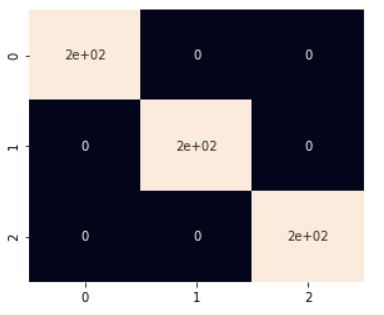
\includegraphics[scale=0.6]{dataset1b_knn_hm_train.jpg}
	\caption{for Training data}
	\label{fig:fig2.2.3.1}
	\end{subfigure}
	\hfill
	\begin{subfigure}[b]{0.45\textwidth}
	\centering
	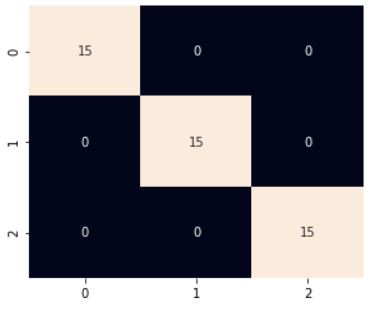
\includegraphics[scale=0.6]{dataset1b_knn_hm_test.jpg}
	\caption{for Test data}
	\label{fig:fig2.2.3.2}
	\end{subfigure}
\caption{Confusion matrix for datatset 1b using KNN classifier,  $K=1$}
\label{fig:fig1.2.1}
\end{figure}

\begin{figure}[h]
\centering
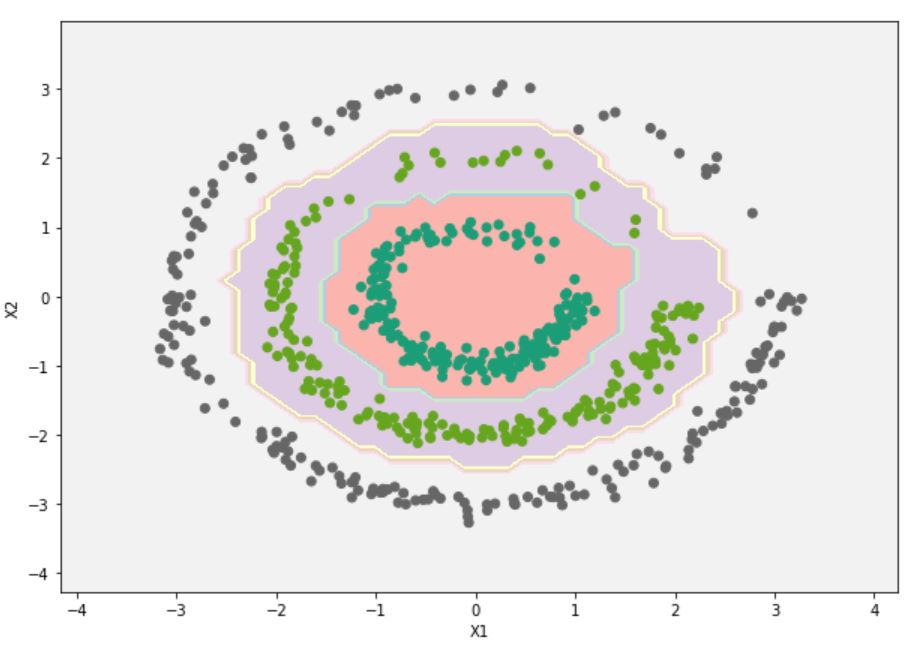
\includegraphics[scale=0.35]{dataset1b_k7_knn.jpg}	
\caption{Decision region plots superposed with training examples for datatset 1b using KNN classifier, $K=1$}
\label{fig:fig2.1.1}
\end{figure}

Although the classes are not linearly separable they are well separated for KNN classifier to give good results.
\newpage
\subsection{Bayes classifier with GMM, using full covariance matrices}
Hyperparameters $Q = \{3,5,10\}$
\begin{table}[h!]
\label{tab:tab1.1.1}
\begin{center}
\begin{tabular}{|l|c|c|c|}
\hline
\textbf{Q } & \textbf{Training Dataset} & \textbf{Validation Dataset} &\textbf{Test Dataset}\\
\hline
$3$ & 91.67 & 97.78 & 91.1\\
\hline
$5$ & 98.66 & 97.78 & 97.78\\
\hline
$10$ & 100 & 100 & 100\\
\hline
\end{tabular}
\caption{Classification accuracy of GMM classifier using full covariance matrix on Dataset 1b}
\end{center}
\end{table}

As we can see from the table above the model with the best performance on the test data is with  Q=10 with an accuracy of 100\% 

\begin{figure}[h]
\centering
	\begin{subfigure}[b]{0.45\textwidth}
	\centering
	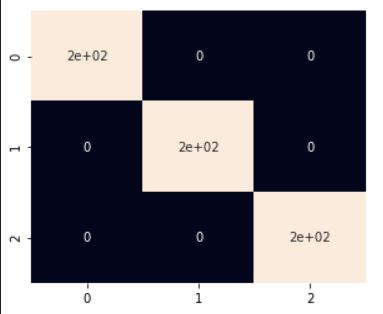
\includegraphics[scale=0.5]{dataset1b_gmm_full_hm_train.jpg}
	\caption{for Training data}
	\label{fig:fig2.2.3.1}
	\end{subfigure}
	\hfill
	\begin{subfigure}[b]{0.45\textwidth}
	\centering
	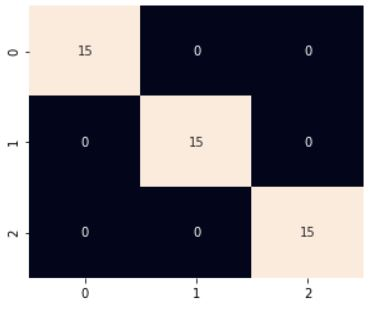
\includegraphics[scale=0.5]{dataset1b_gmm_full_hm_test.jpg}
	\caption{for Test data}
	\label{fig:fig2.2.3.2}
	\end{subfigure}
\caption{Confusion matrix for datatset 1b using GMM with full covariance matrix, $Q= 10$}
\label{fig:fig1.2.1}
\end{figure}
\begin{figure}[h]
\centering
	\begin{subfigure}[b]{0.45\textwidth}
	\centering
	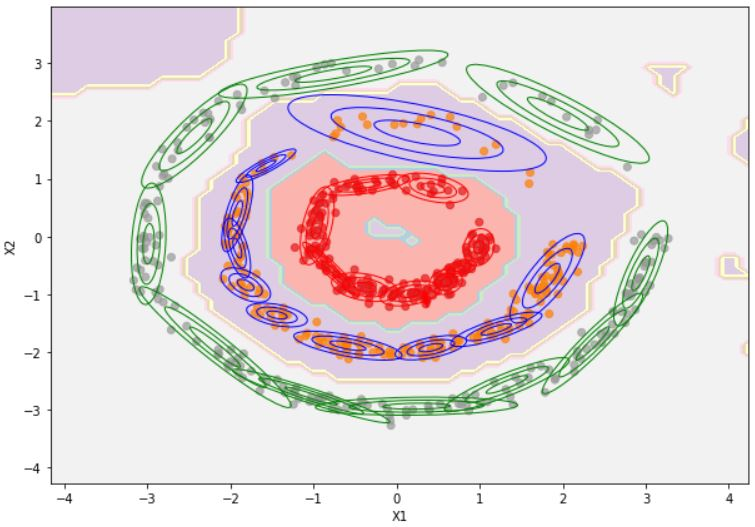
\includegraphics[scale=0.35]{dataset1b_k10_fullC_GMM_2D.jpg}
	\caption{Decision region plots superposed with training examples}
	\label{fig:fig2.2.3.1}
	\end{subfigure}
	\hfill
	\begin{subfigure}[b]{0.45\textwidth}
	\centering
	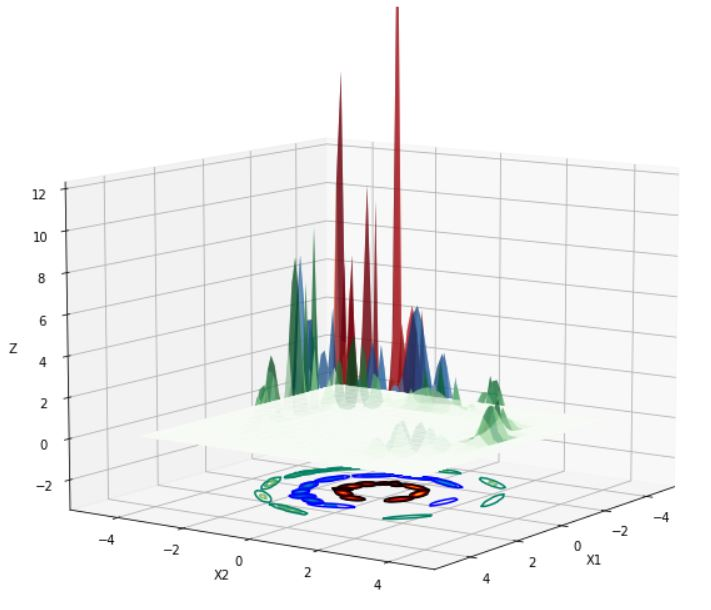
\includegraphics[scale=0.35]{dataset1b_k10_fullC_GMM_3D.jpg}
	\caption{Plots of the level curves}
	\label{fig:fig2.2.3.2}
	\end{subfigure}
\caption{Plots for datatset 1b using GMM with full covariance matrix, $Q= 10$}
\label{fig:fig1.2.1}
\end{figure}

\newpage
\subsection{Bayes classifier with GMM, using diagonal covariance matrices}
Hyperparameters $Q = \{3,5,10\}$
\begin{table}[h!]
\label{tab:tab1.1.1}
\begin{center}
\begin{tabular}{|l|c|c|c|}
\hline
\textbf{Q } & \textbf{Training Dataset} & \textbf{Validation Dataset} &\textbf{Test Dataset}\\
\hline
$3$ & 91.67 & 97.78 & 91.1\\
\hline
$5$ & 98.66 & 97.78 & 97.78\\
\hline
$10$ & 99.67 & 100 & 100\\
\hline
\end{tabular}
\caption{Classification accuracy of GMM classifier using diagonal covariance matrices on Dataset 1b}
\end{center}
\end{table}

As we can see from the table above the model with the best performance on the test data is with  Q=10 with an accuracy of 100\% 

\begin{figure}[h]
\centering
	\begin{subfigure}[b]{0.45\textwidth}
	\centering
	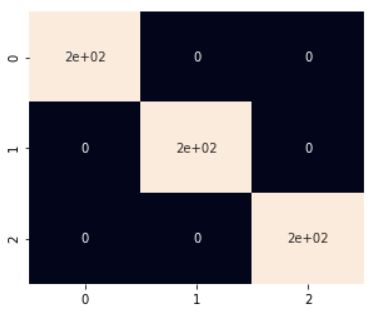
\includegraphics[scale=0.5]{dataset1b_gmm_diagonal_hm_train.jpg}
	\caption{for Training data}
	\label{fig:fig2.2.3.1}
	\end{subfigure}
	\hfill
	\begin{subfigure}[b]{0.45\textwidth}
	\centering
	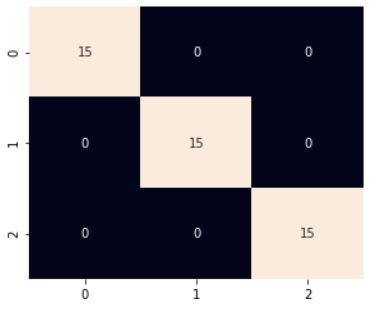
\includegraphics[scale=0.5]{dataset1b_gmm_diagonal_hm_test.jpg}
	\caption{for Test data}
	\label{fig:fig2.2.3.2}
	\end{subfigure}
\caption{Confusion matrix for datatset 1b using GMM classifier with diagonal covariance matrices}
\label{fig:fig1.2.1}
\end{figure}

\begin{figure}[h]
\centering
	\begin{subfigure}[b]{0.45\textwidth}
	\centering
	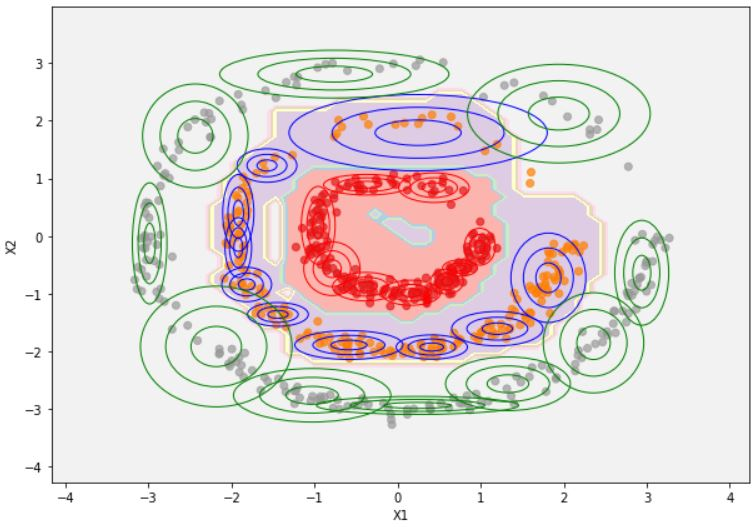
\includegraphics[scale=0.3]{dataset1b_k10_diagonalC_GMM_2D.jpg}
	\caption{Decision region plots superposed with training examples}
	\label{fig:fig2.2.3.1}
	\end{subfigure}
	\hfill
	\begin{subfigure}[b]{0.45\textwidth}
	\centering
	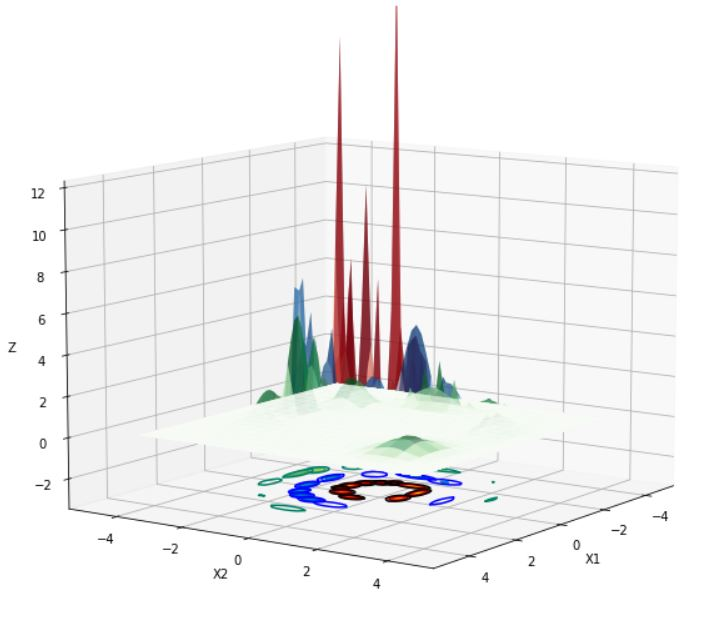
\includegraphics[scale=0.3]{dataset1b_k10_diagonalC_GMM_3D.jpg}
	\caption{Plots of the level curves}
	\label{fig:fig2.2.3.2}
	\end{subfigure}
\caption{Plots for datatset 1b using GMM with diagonal covariance matrix, $Q= 10$}
\label{fig:fig1.2.1}
\end{figure}

We saw that with full covariance matrix we get a slightly better result as compared to the diagonal covariance matrix since the GMMs are not restricted to be aligned with the principal axes.

\newpage
\subsection{Bayes classifier with K-nearest neighbours method for estimation of class-conditional probability density function}

Hyperparameters $K = \{10,20\}$
\begin{table}[h!]
\label{tab:tab1.1.1}
\begin{center}
\begin{tabular}{|l|c|c|c|}
\hline
\textbf{K } & \textbf{Training Dataset} & \textbf{Validation Dataset} &\textbf{Test Dataset}\\
\hline
$10$ & 99.5 & 100 & 100\\
\hline
$20$ & 96 & 100 & 96.56\\
\hline
\end{tabular}
\caption{Classification accuracy of KNN density estimator classifier on Dataset 1b}
\end{center}
\end{table}

As we can see from the table above the model with the best performance on the test data is with  K=10 with an accuracy of 100\% 
\begin{figure}[h]
\centering
	\begin{subfigure}[b]{0.45\textwidth}
	\centering
	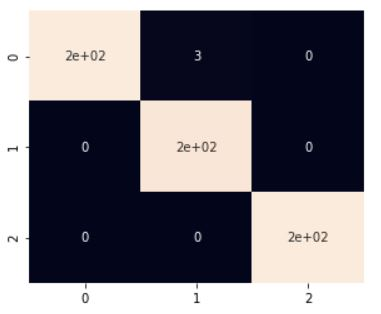
\includegraphics[scale=0.6]{dataset1b_knnde_hm_train.jpg}
	\caption{for Training data}
	\label{fig:fig2.2.3.1}
	\end{subfigure}
	\hfill
	\begin{subfigure}[b]{0.45\textwidth}
	\centering
	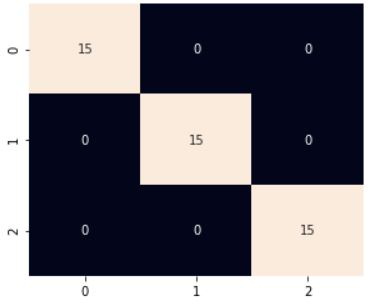
\includegraphics[scale=0.6]{dataset1b_knnde_hm_test.jpg}
	\caption{for Test data}
	\label{fig:fig2.2.3.2}
	\end{subfigure}
\caption{Confusion matrix for datatset 1b using KNN density estimator classifier, $K =10$}
\label{fig:fig1.2.1}
\end{figure}

\begin{figure}[h]
\centering
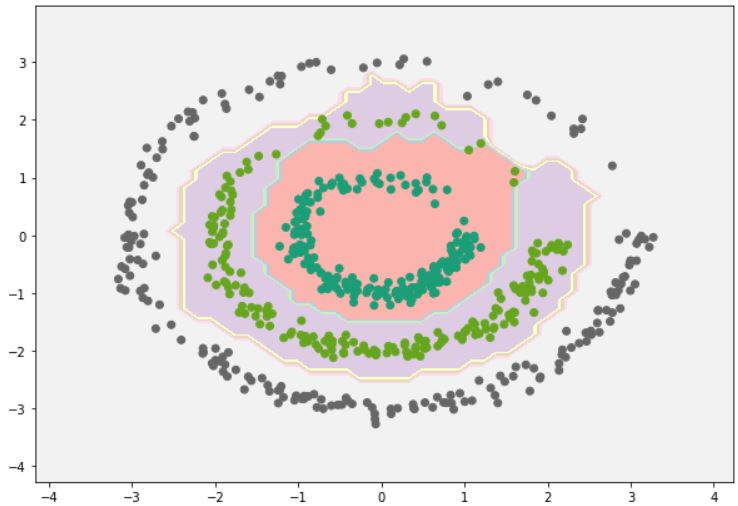
\includegraphics[scale=0.35]{dataset1b_k10_knn_density.jpg}	
\caption{Decision region plots superposed with training examples for datatset 1b using KNN density estimator, $K=10$}
\label{fig:fig2.1.1}
\end{figure}

For KNN using density estimators the decision surface was able to classify better with lesser K as the regions with low density of training points were easily misclassified.
\newpage

\section{Dataset 2a}
\subsection{Bayes classifier with GMM, using full covariance matrices}

The classes we had to distinguish between were:
\begin{enumerate}
\item Forest
\item Highway
\item Inside city
\item Mountain
\item Street
\end{enumerate}

Hyperparameters $Q = \{3,5,10\}$
\begin{table}[h!]
\label{tab:tab1.1.1}
\begin{center}
\begin{tabular}{|l|c|c|c|}
\hline
\textbf{Q } & \textbf{Training Dataset} & \textbf{Validation Dataset} &\textbf{Test Dataset}\\
\hline
$3$ & 68.83 & 54.77 & 55.12\\
\hline
$5$ & 72.04 & 61.14 & 59.61\\
\hline
$10$ & 74.88 & 59.23 & 61.53\\
\hline
\end{tabular}
\caption{Classification accuracy of GMM classifier using full covariance matrices on Dataset 2a}
\end{center}
\end{table}

As we can see from the table above the model with the best performance on the test data is with  Q=10 with an accuracy of 61.53\% 

\begin{figure}[h]
\centering
	\begin{subfigure}[b]{0.45\textwidth}
	\centering
	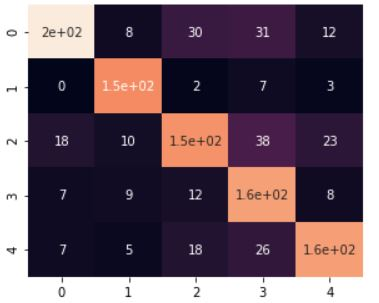
\includegraphics[scale=0.6]{dataset2a_gmm_full_hm_train.jpg}
	\caption{for Training data}
	\label{fig:fig2.2.3.1}
	\end{subfigure}
	\hfill
	\begin{subfigure}[b]{0.45\textwidth}
	\centering
	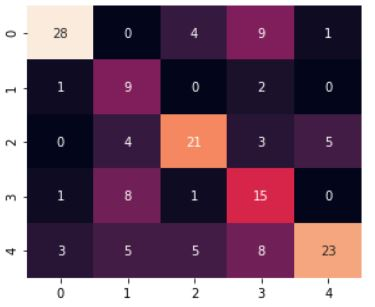
\includegraphics[scale=0.6]{dataset2a_gmm_full_hm_test.jpg}
	\caption{for Test data}
	\label{fig:fig2.2.3.2}
	\end{subfigure}
\caption{Confusion matrix for datatset 2a using GMM with full covariance matrix}
\label{fig:fig1.2.1}
\end{figure}

\newpage
\subsection{Bayes classifier with GMM, using diagonal covariance matrices}

Hyperparameters $Q = \{3,5,10\}$
\begin{table}[h!]
\label{tab:tab1.1.1}
\begin{center}
\begin{tabular}{|l|c|c|c|}
\hline
\textbf{Q } & \textbf{Training Dataset} & \textbf{Validation Dataset} &\textbf{Test Dataset}\\
\hline
$3$ & 69.29 & 56.68 & 57.05\\
\hline
$5$ & 72.86 & 60.50 & 59.61\\
\hline
$10$ & 76.35 & 60.50 & 62.17\\
\hline
\end{tabular}
\caption{Classification accuracy of GMM classifier using diagonal covariance matrices on Dataset 2a}
\end{center}
\end{table}

As we can see from the table above the model with the best performance on the test data is with  Q=10 with an accuracy of 62.17\% 

\begin{figure}[h]
\centering
	\begin{subfigure}[b]{0.45\textwidth}
	\centering
	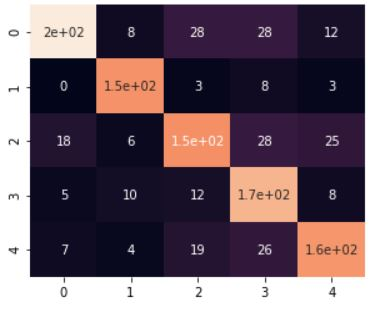
\includegraphics[scale=0.6]{dataset2a_gmm_diagonal_hm_train.jpg}
	\caption{for Training data}
	\label{fig:fig2.2.3.1}
	\end{subfigure}
	\hfill
	\begin{subfigure}[b]{0.45\textwidth}
	\centering
	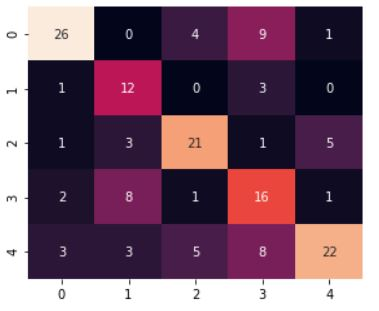
\includegraphics[scale=0.6]{dataset2a_gmm_diagonal_hm_test.jpg}
	\caption{for Test data}
	\label{fig:fig2.2.3.2}
	\end{subfigure}
\caption{Confusion matrix for datatset 2a using GMM with diagonal covariance matrix}
\label{fig:fig1.2.1}
\end{figure}

For the real dataset the GMM with higher number of clusters was also unable to classify the examples with very high accuracy. \\
As we increased the number of clusters the accuracy increased to a point after which we started getting some empty clusters as well during the model training.
We added an epsilon value to the covariance matrices to ensure that they don't become singular.
\newpage

\section{Dataset 2b}
\subsection{Bayes classifier with GMM, using full covariance matrices}

The classes we had to distinguish between were:
\begin{enumerate}
\item Forest
\item Highway
\item Inside city
\item Mountain
\item Street
\end{enumerate}

Hyperparameters $Q = \{3,7,13\}$
\begin{table}[h!]
\label{tab:tab1.1.1}
\begin{center}
\begin{tabular}{|l|c|c|c|}
\hline
\textbf{Q } & \textbf{Training Dataset} & \textbf{Validation Dataset} &\textbf{Test Dataset}\\
\hline
$3$ & 68.10 & 69.42 & 71.79\\
\hline
$7$ & 74.61 & 72.61 & 70.51\\
\hline
$13$ & 73.78 & 74.52 & 71.79\\
\hline
\end{tabular}
\caption{Classification accuracy of GMM classifier using full covariance matrices on Dataset 2b}
\end{center}
\end{table}

As we can see from the table above the model with the best performance on the test data is with  Q=13 with an accuracy of 71.79\% 

\begin{figure}[h]
\centering
	\begin{subfigure}[b]{0.45\textwidth}
	\centering
	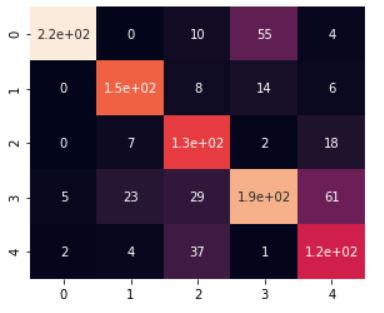
\includegraphics[scale=0.6]{dataset2b_gmm_full_hm_train.jpg}
	\caption{for Training data}
	\label{fig:fig2.2.3.1}
	\end{subfigure}
	\hfill
	\begin{subfigure}[b]{0.45\textwidth}
	\centering
	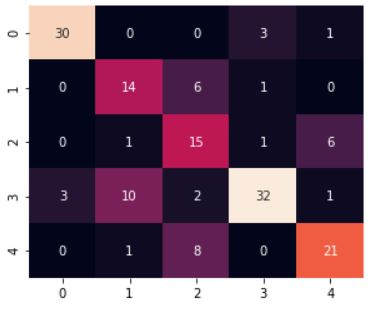
\includegraphics[scale=0.6]{dataset2b_gmm_full_hm_test.jpg}
	\caption{for Test data}
	\label{fig:fig2.2.3.2}
	\end{subfigure}
\caption{Confusion matrix for datatset 2b using GMM classifier with full covariance matrices}
\label{fig:fig1.2.1}
\end{figure}

\newpage
\subsection{Bayes classifier with GMM, using diagonal covariance matrices}

Hyperparameters $Q = \{3,7,13\}$
\begin{table}[h!]
\label{tab:tab1.1.1}
\begin{center}
\begin{tabular}{|l|c|c|c|}
\hline
\textbf{Q } & \textbf{Training Dataset} & \textbf{Validation Dataset} &\textbf{Test Dataset}\\
\hline
$3$ & 65.99 & 69.42 & 67.94\\
\hline
$7$ & 73.69  & 69.42 & 73.71\\
\hline
$13$ & 73.69 & 73.24 & 74.35\\
\hline
\end{tabular}
\caption{Classification accuracy of GMM classifier using diagonal covariance matrices on Dataset 2b}
\end{center}
\end{table}

As we can see from the table above the model with the best performance on the test data is with  Q=13 with an accuracy of 74.35\% 

\begin{figure}[h]
\centering
	\begin{subfigure}[b]{0.45\textwidth}
	\centering
	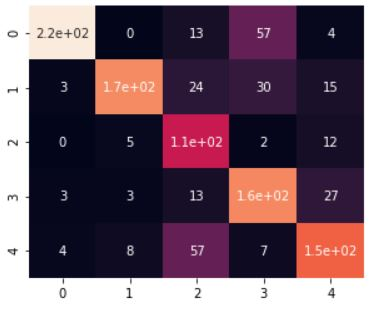
\includegraphics[scale=0.6]{dataset2b_gmm_diagonal_hm_train.jpg}
	\caption{for Training data}
	\label{fig:fig2.2.3.1}
	\end{subfigure}
	\hfill
	\begin{subfigure}[b]{0.45\textwidth}
	\centering
	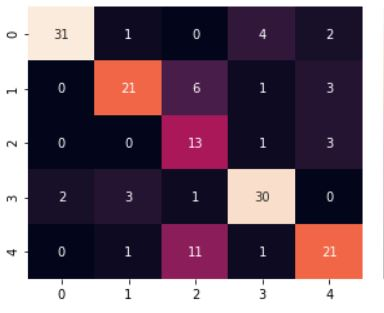
\includegraphics[scale=0.6]{dataset2b_gmm_diagonal_hm_test.jpg}
	\caption{for Test data}
	\label{fig:fig2.2.3.2}
	\end{subfigure}
\caption{Confusion matrix for datatset 2b using GMM classifier with diagonal covariance matrices}
\label{fig:fig1.2.1}
\end{figure}

We faced similar issues with this dataset as well but since we had more training data ($36X$) of the previous example we could increase the number of clusters to a higher point to get better classification accuracy.

\end{document}
